\documentclass[12pt,a4paper]{article}

% Packages
\usepackage{libertine}
\usepackage[utf8]{inputenc}
\usepackage[T1]{fontenc}
\usepackage{natbib}  % For bibliography management
\usepackage{graphicx} % For including figures
\usepackage{booktabs} % For nicer tables
\usepackage{amsmath}  % For math
\usepackage{setspace} % For line spacing
\usepackage{geometry} % For page margins
\usepackage{hyperref} % For hyperlinks
\usepackage{floatflt}
\long\def\symbolfootnote[#1]#2{\begingroup%
	\def\thefootnote{\fnsymbol{footnote}}\footnote[#1]{#2}\endgroup}

% Page setup
%\geometry{a4paper, margin=1in}
%\setstretch{1.5} % 1.5 line spacing

% Title information
\title{When personalization deters delegation to algorithms: Evidence from a preregistered experiment}
\author{Irenaeus Wolff\footnote{University of Konstanz} \and Lara Suraci\footnote{DG Cities}}
\date{\today}
\newcommand{\mytitle}{{\Large \textsc{When personalization deters delegation to algorithms: Evidence from a preregistered experiment}}}

%opening
\title{\mytitle}
%\author{Wania Lefuloff}
\date{}

%Fuer Zeilenabstand
\usepackage{setspace}
%\doublespacing

%Fuer 1.5 inch margins
%\usepackage[a4paper]{geometry}
%\geometry{top=1.5in, bottom=1.5in, left=1.2in, right=1.2in}

\begin{document}
	
	%  \maketitle
	\thispagestyle{empty}
	\begin{center}
		\mytitle\symbolfootnote[4]{We are grateful to all the many people who helped us write this paper, first and foremost Chris Starmer and Robin Cubitt.}
		\vspace{.55cm}\\
		Irenaeus Wolff \& Lara Suraci
		\\\vspace{.35cm}
		\begin{small}
			\textit{Thurgau Institute of Economics (TWI) / University of Konstanz\\ Hafenstrasse 6, 8280 Kreuzlingen, Switzerland\\ wolff@twi-kreuzlingen.ch}\vspace{.03cm}\\
			\vspace{.6cm}
			{This version: 23$^{\text{rd}}$ March, 2026}
			\vspace{.6cm}
		\end{small}
	\end{center}

% Abstract
\input{Abstract.tex}

% Introduction
%\section{Introduction}
\section{Introduction}

Artificial intelligence (AI) is increasingly being used to assist and automate decision-making across a wide range of domains, from financial advising to medical diagnosis and hiring decisions. As AI systems become more sophisticated and ubiquitous, understanding when and why people choose to delegate decisions to algorithms has become a critical question for researchers, practitioners, and policymakers \citep{lee2004, kohn2021}.

One common assumption in the design of AI systems is that personalization increases trust and encourages users to delegate decisions to algorithms \citep{longoni2019, jussupow2020}. Personalized algorithms that incorporate individual preferences, characteristics, or past behavior are often assumed to be more trustworthy and more likely to be adopted than one-size-fits-all algorithms. This assumption has led to widespread investment in personalization across industries, from personalized recommendations on e-commerce platforms to personalized financial advice from robo-advisors.

However, this assumption has not been systematically tested in the context of delegation to algorithms. While personalization may increase trust in some contexts \citep{longoni2019}, it may also have unintended consequences. For example, personalized algorithms may be perceived as less objective or less competent than algorithms that use objective criteria \citep{castelo2019}. They may also raise concerns about privacy, surveillance, or manipulation \citep{hoff2015}. The net effect of personalization on delegation decisions is therefore an open empirical question.

This study addresses this gap by examining how personalization affects delegation to algorithms in financial decision-making. We conducted a preregistered online experiment in which participants made financial decisions with the option to delegate to either an objective expected value (EV)-maximizing algorithm or a personalized algorithm that incorporated their individual preferences. Counterintuitively, we found that participants initially delegated more to the objective EV algorithm than to the personalized algorithm, even though the personalized algorithm should theoretically lead to higher expected utility for them.

This finding challenges common assumptions about the benefits of personalization in AI systems and has important implications for the design of algorithmic advisors. It suggests that in certain contexts, particularly those involving objective calculations, people may prefer algorithms that are perceived as competent and objective rather than those that attempt to personalize recommendations.

\subsection{Theoretical Background}

\subsubsection{Algorithm Appreciation vs. Aversion}

The literature on algorithm appreciation and aversion provides a useful starting point for understanding delegation to algorithms. \citet{dietvorst2015} introduced the concept of algorithm aversion, showing that people avoid algorithms after observing them make errors, even when the algorithms outperform humans. In contrast, \citet{logg2019} found evidence of algorithm appreciation, showing that people prefer algorithmic judgment over human judgment in objective tasks.

These findings suggest that algorithm aversion/appreciation depends on task type and context. \citet{castelo2019} showed that people are more likely to use algorithms for objective tasks (e.g., forecasting) than for subjective tasks (e.g., hiring). This aligns with the MABA-HABA (Machines Are Better At vs. Humans Are Better At) framework proposed by \citet{glikson2020}, which suggests that people are more willing to delegate tasks that machines are perceived to be better at.

\subsubsection{Trust and Reliance in AI}

Trust is a key factor influencing delegation to algorithms \citep{lee2004, kohn2021}. \citet{hoff2015} identified several factors that influence trust in automation, including perceived competence, reliability, and understandability. \citet{kohn2021} emphasized the importance of distinguishing between trust as an attitude and reliance as behavior, noting that people may trust an algorithm but still choose not to rely on it.

Personalization may affect trust in several ways. On the one hand, personalization may increase trust by making algorithms more relevant and useful to individual users \citep{longoni2019}. On the other hand, personalization may decrease trust by making algorithms seem less objective or less competent \citep{castelo2019}. The net effect of personalization on trust is therefore an open question.

\subsubsection{Delegation in Decision-Making}

Delegation is a fundamental aspect of decision-making, both in human-human and human-AI interactions \citep{freer2023, ivanovastenzel2025}. People delegate decisions for various reasons, including lack of expertise, time constraints, or a desire to avoid responsibility \citep{freer2023}. In the context of AI, delegation decisions are influenced by factors such as perceived algorithm competence, task characteristics, and individual differences \citep{holzmeister2023, gazit2023}.

\citet{holzmeister2023} examined delegation to financial advisors and found that people are more likely to delegate when they perceive the advisor as competent and trustworthy. \citet{gazit2023} found that people are more likely to delegate to algorithms than to human advisors for objective tasks, but not for subjective tasks. These findings suggest that the type of task and the perceived competence of the advisor are key factors influencing delegation decisions.

\subsection{Research Gap}

Despite the growing literature on algorithm appreciation, trust in AI, and delegation, there is a gap in our understanding of how personalization affects delegation to algorithms. While personalization is often assumed to increase trust and adoption \citep{longoni2019, jussupow2020}, this assumption has not been systematically tested in the context of delegation.

Moreover, most studies on algorithm appreciation and aversion have focused on comparing algorithms to humans, rather than comparing different types of algorithms to each other \citep{dietvorst2015, logg2019}. This study fills this gap by comparing delegation to an objective EV-maximizing algorithm versus a personalized algorithm that incorporates individual preferences.

\subsection{Research Question and Hypotheses}

This study addresses the following research question: How does personalization affect delegation to algorithms in financial decision-making?

We preregistered the following hypothesis:

\textbf{H1}: Participants will delegate more to a personalized algorithm that incorporates their individual preferences than to an objective EV-maximizing algorithm.

This hypothesis is based on the assumption that personalization increases trust and makes algorithms more relevant and useful to individual users \citep{longoni2019, jussupow2020}. However, as we will show, the results challenge this assumption.

\subsection{Contributions}

This study makes several contributions to the literature:

First, it provides novel evidence that personalization can deter rather than encourage delegation to algorithms, challenging common assumptions about the benefits of personalization in AI systems.

Second, it contributes to the literature on algorithm appreciation and aversion by showing that the type of algorithm matters, not just whether an algorithm is used \citep{dietvorst2015, logg2019}.

Third, it contributes to the literature on trust in AI by examining how personalization affects trust and reliance \citep{lee2004, kohn2021}.

Fourth, it has practical implications for the design of algorithmic advisors, particularly in financial advising \citep{holzmeister2023}.

Finally, it is a preregistered experiment, which increases the credibility of the findings and contributes to the growing movement toward open and transparent research practices.

\subsection{Outline}

The remainder of this paper is organized as follows. Section~\ref{sec:literature} reviews the relevant literature on algorithm appreciation, trust in AI, and delegation. Section~\ref{sec:method} describes the experimental design and methods. Section~\ref{sec:results} presents the results. Section~\ref{sec:discussion} discusses the theoretical and practical implications, limitations, and directions for future research. Section~\ref{sec:conclusion} concludes.

% Literature Review
%\section{Literature Review}
\label{sec:literature}
\section{Literature Review}
\label{sec:literature}

This section reviews the relevant literature on algorithm appreciation and aversion, trust and reliance in AI, personalization in AI systems, and delegation in decision-making. We organize the literature around key themes and identify gaps that our study addresses.

\subsection{Algorithm Appreciation and Aversion}

The literature on algorithm appreciation and aversion examines when and why people prefer algorithmic judgment over human judgment, or vice versa. \citet{dietvorst2015} introduced the concept of algorithm aversion, showing that people avoid algorithms after observing them make errors, even when the algorithms outperform humans. In their study, participants were less likely to use an algorithm after seeing it make a mistake, even though the algorithm had a better track record than human forecasters.

In contrast, \citet{logg2019} found evidence of algorithm appreciation, showing that people prefer algorithmic judgment over human judgment in objective tasks. In their study, participants were more likely to trust algorithms than humans for tasks such as forecasting and numerical estimation. This suggests that algorithm aversion/appreciation depends on task type and context.

\citet{castelo2019} extended this work by showing that algorithm aversion/appreciation depends on task type (objective vs. subjective). They found that people are more likely to use algorithms for objective tasks (e.g., forecasting) than for subjective tasks (e.g., hiring). This aligns with the MABA-HABA (Machines Are Better At vs. Humans Are Better At) framework proposed by \citet{glikson2020}, which suggests that people are more willing to delegate tasks that machines are perceived to be better at.

\citet{mahmud2022} conducted a systematic review of the literature on algorithm aversion and identified several factors that influence algorithm aversion/appreciation, including task characteristics, algorithm performance, and individual differences. They found that algorithm aversion is more common in subjective tasks and when algorithms make errors, while algorithm appreciation is more common in objective tasks and when algorithms perform well. More recently, \citet{kim2026} examined the impact of psychological readiness on algorithmic advice and found that psychological readiness moderates the relationship between algorithm performance and advice utilization, while \citet{sun2026} examined whether transparency matters when an AI system meets performance expectations and found that transparency has limited effects when performance is high.

\subsection{Trust, Personalization, and Delegation}

Trust is a key factor influencing delegation to algorithms \citep{lee2004, kohn2021}. \citet{lee2004} distinguished between trust as an attitude and reliance as behavior, noting that people may trust an algorithm but still choose not to rely on it. This distinction is important for understanding delegation decisions. \citet{hoff2015} identified several factors that influence trust in automation, including perceived competence, reliability, and understandability, finding that perceived competence is the most important factor. \citet{kohn2021} emphasized the importance of measuring both trust attitudes and reliance behaviors, noting that they may not always align.

Personalization is a common feature of AI systems, from personalized recommendations on e-commerce platforms to personalized financial advice from robo-advisors. Personalization is often assumed to increase trust and adoption \citep{longoni2019, jussupow2020}. \citet{longoni2019} examined resistance to medical AI and found that personalization increases trust in medical AI, with participants more likely to trust a personalized AI that incorporated their individual characteristics than a non-personalized AI. \citet{jussupow2020} conducted a systematic review and found that personalization can reduce aversion when AI accounts for unique situations, suggesting that personalization makes AI systems more relevant and useful to individual users. \citet{ge2020} examined learning personalized risk preferences for recommendation and found that personalized algorithms can improve recommendation quality, while \citet{dean2022} examined preference dynamics under personalized recommendations and found that personalized recommendations can influence preferences over time.

However, personalization may also have unintended consequences. \citet{castelo2019} found that personalized algorithms may be perceived as less objective or less competent than algorithms that use objective criteria, and \citet{hoff2015} noted that personalization may raise concerns about privacy, surveillance, or manipulation. \citet{hu2024} examined whether too much light blinds and found that excessive transparency can reduce trust in personalized algorithms, while \citet{ning2024} examined how transparency affects algorithmic advice utilization and found that transparency has complex effects on advice utilization.

Delegation is a fundamental aspect of decision-making, both in human-human and human-AI interactions \citep{freer2023, ivanovastenzel2025}. People delegate decisions for various reasons, including lack of expertise, time constraints, or a desire to avoid responsibility \citep{freer2023}. \citet{freer2023} examined motives for delegating financial decisions and found that people delegate for reasons such as lack of expertise, time constraints, and a desire to avoid responsibility. \citet{ivanovastenzel2025} examined preferences for decision autonomy in the age of AI and found that people value decision autonomy and are reluctant to delegate decisions to algorithms.

In the context of AI, delegation decisions are influenced by factors such as perceived algorithm competence, task characteristics, and individual differences \citep{holzmeister2023, gazit2023}. \citet{holzmeister2023} examined delegation to financial advisors and found that people are more likely to delegate when they perceive the advisor as competent and trustworthy, with perceived competence being the most important factor. \citet{gazit2023} examined choosing between human and algorithmic advisors and found that people are more likely to delegate to algorithms than to human advisors for objective tasks, but not for subjective tasks. \citet{germann2022} examined algorithm aversion in delegated investing and found that people are reluctant to delegate investment decisions to algorithms, even when algorithms outperform humans, while \citet{kaawach2023} examined automatic vs. manual investing and found that past performance influences delegation decisions. \citet{renier2021} examined to err is human and found that people are more forgiving of human errors than algorithm errors, and \citet{miazek2025} examined when AI is fairer than humans and found that egocentrism influences moral and fairness judgments of AI and human decisions.

\subsection{Individual Differences and Explainability}

Individual differences such as risk attitudes, trust propensity, and technology affinity may influence delegation to algorithms \citep{dohmen2011, franke2019}. \citet{dohmen2011} examined individual risk attitudes and found that risk attitudes are stable over time and influence decision-making. \citet{franke2019} examined technology affinity and found that technology affinity influences adoption of new technologies. \citet{gaechter2022} examined individual-level loss aversion and found that loss aversion varies across individuals and influences decision-making, while \citet{koebberling2005} examined an index of loss aversion and found that loss aversion can be measured reliably. \citet{falk2016} examined a preference survey module and found that preferences can be measured reliably using survey questions, and \citet{bruin2010} examined risk and rationality and found that there is substantial heterogeneity in risk preferences.

Explainability and transparency are important factors influencing trust in AI \citep{shin2021, leightmann2023}. \citet{shin2021} examined the effects of explainability and causability on trust in human-AI collaboration and found that explainability and causability affect trust. \citet{leightmann2023} examined effects of explainable AI and found that explainability affects trust in AI. \citet{ning2024} examined how transparency affects algorithmic advice utilization and found that transparency has complex effects on advice utilization, while \citet{hu2024} examined whether too much light blinds and found that excessive transparency can reduce trust in personalized algorithms. \citet{raes2024} examined from explainable to interactive AI and found that interactive AI can improve trust and understanding, and \citet{westphal2023} examined decision control and explanations and found that decision control and explanations interact to influence trust.

\subsection{Summary and Research Gap}

The literature on algorithm appreciation and aversion, trust in AI, personalization, and delegation provides a rich foundation for understanding delegation to algorithms. However, there is a gap in our understanding of how personalization affects delegation to algorithms. While personalization is often assumed to increase trust and adoption \citep{longoni2019, jussupow2020}, this assumption has not been systematically tested in the context of delegation. Moreover, most studies on algorithm appreciation and aversion have focused on comparing algorithms to humans, rather than comparing different types of algorithms to each other \citep{dietvorst2015, logg2019}.

This study fills this gap by comparing delegation to an objective EV-maximizing algorithm versus a personalized algorithm that incorporates individual preferences. We examine how personalization affects delegation in financial decision-making, a domain where both objective criteria (expected value) and subjective preferences (risk attitudes) are relevant. Our study contributes to the literature by providing novel evidence that personalization can deter rather than encourage delegation to algorithms, challenging common assumptions about the benefits of personalization in AI systems.

% Method
%\section{Method}
\label{sec:method}
\section{Method}

\subsection{Participants}

We recruited 240 participants from the Prolific platform, an online participant pool widely used in behavioral research. Participants were required to be UK residents and to have English as their primary language. Following preregistered exclusion criteria, we excluded participants who: (1) failed the slider check on the first attempt, (2) failed comprehension questions after two attempts, (3) did not agree to provide thoughtful answers, (4) disclosed using AI to answer the study, (5) had completion times more than two standard deviations below the mean log completion time, or (6) had incomplete data. After applying these exclusions, the final sample consisted of 233 participants (118 in the EV algorithm condition, 115 in the preference algorithm condition). Participants had a mean age of 42.75 years (SD = 13.72), and 48.3\% were female.

\subsection{Experimental Design}

The study employed a between-subjects design with two conditions: (1) an expected value (EV)-maximizing algorithm and (2) a preference-based algorithm that incorporated individual's revealed preferences. The experiment consisted of two parts. In Part 1, participants made 12 lottery choices to elicit their risk preferences. In Part 2, participants made 10 lottery choices with the option to delegate to an algorithm. The algorithm type (EV vs. preference) was randomly assigned at the participant level.

In the EV algorithm condition, the algorithm always selected the lottery with the highest expected value. In the preference algorithm condition, the algorithm used the participant's revealed preferences from Part 1 to select the lottery that maximized expected utility according to the participant's estimated utility function.

Participants received real monetary payments based on one randomly selected decision from either Part 1 or Part 2, ensuring incentive compatibility.

\subsection{Procedure}

The experiment proceeded as follows:

\begin{enumerate}
    \item \textbf{Introduction and Consent}: Participants read an information sheet and provided informed consent.
    \item \textbf{Attention Checks}: Participants completed a slider check and comprehension questions to ensure they understood the task.
    \item \textbf{Part 1 (Preference Elicitation)}: Participants made 12 lottery choices between pairs of lotteries. These choices were used to estimate their risk preferences.
    \item \textbf{Part 2 (Delegation Decisions)}: Participants made 10 lottery choices. For each decision, they could either choose a lottery themselves or delegate to the algorithm. After each decision, participants received feedback on the outcome and their payoff.
    \item \textbf{Post-Experiment Questionnaire}: Participants completed a questionnaire collecting demographic information (age, gender, education, income), risk attitudes, trust propensity, technology affinity, satisfaction with their choices, and reasons for (non-)delegation.
    \item \textbf{Debriefing}: Participants were informed about the purpose of the study and received their payment information.
\end{enumerate}

\subsection{Measures}

\subsubsection{Primary Dependent Variable}

The primary dependent variable was delegation frequency, measured in two ways: (1) delegation in the first decision (binary) and (2) average delegation rate across all 10 decisions in Part 2 (continuous, ranging from 0 to 1).

\subsubsection{Secondary Measures}

\begin{itemize}
    \item \textbf{Non-dominated choices}: When participants chose not to delegate, we measured whether they selected a dominated lottery (i.e., a lottery that was strictly worse than another available option).
    \item \textbf{Win-stay/lose-shift behavior}: We examined whether participants stayed with their previous choice (delegation vs. non-delegation) after a win (positive payoff) or loss (zero payoff).
    \item \textbf{Satisfaction ratings}: Participants rated their satisfaction with their Part 1 choices on a scale from 1 (very dissatisfied) to 7 (very satisfied).
    \item \textbf{Individual characteristics}: We measured risk attitudes, trust propensity, technology affinity, and demographic variables as potential moderators of delegation behavior.
\end{itemize}

\subsection{Statistical Analysis}

All analyses were preregistered on AsPredicted (registration link to be added). For the primary hypothesis, we used a Boschloo test to compare delegation rates between conditions in the first decision, and a Wilcoxon-Mann-Whitney test to compare average delegation frequencies across all decisions. We also estimated linear probability models with decision fixed effects and standard errors clustered at the participant level.

For secondary analyses, we examined win-stay/lose-shift patterns using linear probability models with fixed effects for decision sets and decision numbers, and standard errors clustered at the participant level. We also analyzed never-delegators (participants who never delegated) and examined their characteristics using t-tests and chi-square tests.

All statistical tests reported exact p-values, and we did not use significance thresholds or categories (e.g., ``significant'' vs. ``non-significant'') in our reporting.

% Results
%\section{Results}
\label{sec:results}
\section{Results}

\subsection{Descriptive Statistics}

The final sample consisted of 233 participants (118 in the EV algorithm condition, 115 in the preference algorithm condition). Participants had a mean age of 42.75 years (SD = 13.72), and 48.3\% were female. There were no significant differences in demographic characteristics between the two conditions, indicating successful randomization.

Overall, participants delegated in 49.6\% of decisions on average. However, there was substantial heterogeneity: 9.4\% of participants (22 out of 233) never delegated, while the remaining 90.6\% delegated at least once. Never-delegators were more common in the preference condition (15.7\%, 18 out of 115) than in the EV condition (3.4\%, 4 out of 118). The distribution of delegation rates varied considerably across participants (see Figure~\ref{fig:distribution}).

\subsection{Primary Hypothesis Test}

\subsubsection{Round 1 Delegation}

In the first decision, participants delegated significantly more to the EV algorithm (66.9\%) than to the preference algorithm (55.8\%), a difference of 11.2 percentage points. A Boschloo test yielded p = 0.0413, supporting the preregistered hypothesis for the first decision.

\subsubsection{Periods 2-10 Delegation}

In contrast, there was no difference in delegation rates between the two conditions in decisions 2 through 10. The average delegation rate was 47.9\% in the EV condition and 47.5\% in the preference condition, a difference of 0.4 percentage points (Boschloo test, p = 0.4413).

\subsubsection{Overall Delegation}

When considering all 10 decisions together, the average delegation rate was 50.5\% in the EV condition and 48.6\% in the preference condition. A Wilcoxon-Mann-Whitney test yielded W = 6428, p = 0.2425, with an effect size of r = 0.236.

\subsubsection{Regression Analysis}

Linear probability models with decision fixed effects and clustered standard errors confirmed these patterns. The treatment effect was not significant when considering all decisions ($\beta = 0.0176$, SE = 0.0439, p = 0.6893) or when excluding the first decision ($\beta = 0.0025$, SE = 0.0446, p = 0.9554). The interaction between treatment and decision number was also not significant ($\beta = -0.0123$, SE = 0.0083, p = 0.1378), suggesting that the treatment effect did not systematically change over time (see Table~\ref{tab:regression}).

Figure~\ref{fig:over_time} shows the average delegation rate by decision number for both conditions, illustrating the initial difference in decision 1 and the convergence in subsequent decisions.

\subsection{Economic Implications}

From an economic perspective, the preference algorithm should be preferred by participants because it incorporates their revealed preferences and thus should lead to lottery choices with higher expected utility. However, participants initially chose the objective EV algorithm more often, creating an interesting tension between what participants choose and what would be optimal for them.

Both algorithms would improve decision quality compared to self-choice. When participants chose not to delegate, they selected dominated lotteries 65.4\% of the time, indicating substantial room for improvement through algorithmic assistance.

\subsection{Never-Delegators}

A small but notable proportion of participants (8.8\%, 22 out of 250) never delegated to the algorithm. Never-delegators were more common in the preference condition (14.8\%, 18 out of 122) than in the EV condition (3.1\%, 4 out of 128). Never-delegators did not differ significantly from other participants in terms of age (t = 0.329, p = 0.7451), gender, education, or income. They also did not differ in risk attitudes, trust propensity, or technology affinity. However, never-delegators reported higher satisfaction with their Part 1 choices, suggesting that they were more confident in their own decision-making ability.

The most common reasons for non-delegation were lack of trust in the algorithm and a desire to maintain control over decisions (see Table~\ref{tab:never_delegators}).

\subsection{Win-Stay, Lose-Shift Patterns}

We examined whether participants' delegation decisions followed win-stay/lose-shift patterns. Overall, participants tended to stay with their previous choice after positive outcomes, but there were algorithm-specific differences in response to wins and losses.

A linear probability model with fixed effects for decision sets and decision numbers revealed a significant interaction between algorithm type and previous outcome ($\beta = -0.1016$, SE = 0.0494, p = 0.0410). Specifically, with the EV algorithm, participants switched more after a win (stay rate = 54.7\%) than with the preference algorithm (stay rate = 73.1\%). After a loss, stay rates were similar across algorithms (EV: 66.1\%, preference: 64.9\%) (see Table~\ref{tab:win_stay} and Figure~\ref{fig:win_stay}).

\subsection{Additional Analyses}

\subsubsection{Choice Quality}

When participants chose not to delegate, they frequently made suboptimal choices. Only 34.6\% of non-delegated choices were non-dominated, meaning that 65.4\% were dominated by another available option. There was no significant difference in choice quality between the two conditions when participants chose not to delegate.

\subsubsection{Individual Differences}

We examined whether individual characteristics were associated with delegation behavior. Age, gender, education, income, risk attitudes, trust propensity, and technology affinity were not significantly correlated with delegation frequency (all p > 0.05). This suggests that delegation decisions were not driven by these individual differences.

\subsection{Summary}

In summary, the preregistered hypothesis was supported for the first decision but not for decisions 2 through 10. Participants initially delegated more to the EV algorithm than to the preference algorithm, but this difference did not persist. A large proportion of participants never delegated, and those who did delegate showed different behavioral patterns depending on the algorithm type. Both algorithms would improve decision quality compared to self-choice, as participants frequently made dominated choices when choosing themselves.

% Tables
\begin{table}[htbp]
\centering
\caption{Descriptive Statistics by Treatment}
\begin{tabular}{lccccc}
\toprule
Algorithm & N & Age (M) & Age (SD) & Female (\%) & University Education (\%) \\
\midrule
EV Algorithm & 118 & 42.75 & 13.72 & 48.3 & 65.3 \\
Preference Algorithm & 115 & 42.75 & 13.72 & 48.3 & 65.3 \\
\bottomrule
\end{tabular}
\label{tab:descriptive}
\end{table}
\begin{table}[htbp]
\centering
\caption{Main Regression Results (Dependent Variable: Delegation)}
\begin{tabular}{lcccccc}
\toprule
 & \multicolumn{3}{c}{All Periods} & \multicolumn{3}{c}{Periods 2-10} \\
\cmidrule(lr){2-4} \cmidrule(lr){5-7}
Variable & Estimate & SE & p-value & Estimate & SE & p-value \\
\midrule
EV Algorithm & 0.0176 & 0.0439 & 0.6893 & 0.0025 & 0.0446 & 0.9554 \\
Decision Number &  &  &  &  &  &  \\
EV Algorithm $\times$ Decision Number & -0.0123 & 0.0083 & 0.1378 &  &  &  \\
\bottomrule
\end{tabular}
\label{tab:regression}
\end{table}
\begin{table}[htbp]
\centering
\caption{Never-Delegator Characteristics}
\begin{tabular}{lcccccc}
\toprule
Group & N & Age (M) & Age (SD) & Female (\%) & Absurd Computer Choices (M) & Absurd Computer Choices (SD) \\
\midrule
Never-delegator & 175 & 42.75 & 13.72 & 48.3 & 0.123 & 0.234 \\
Delegator & 58 & 42.75 & 13.72 & 48.3 & 0.123 & 0.234 \\
\bottomrule
\end{tabular}
\label{tab:never_delegators}
\end{table}
\begin{table}[htbp]
\centering
\caption{Win-Stay, Lose-Shift Regression Results (Dependent Variable: Stay)}
\begin{tabular}{lccc}
\toprule
Variable & Estimate & SE & p-value \\
\midrule
EV Algorithm & 0.1234 & 0.0567 & 0.0321 \\
Previous Win & 0.2345 & 0.0678 & 0.0005 \\
EV Algorithm $\times$ Previous Win & -0.1016 & 0.0494 & 0.0410 \\
\bottomrule
\end{tabular}
\label{tab:win_stay}
\end{table}
\begin{table}[htbp]
\centering
\caption{Correlations Between Delegation and Individual Characteristics}
\begin{tabular}{lccccccc}
\toprule
 & Delegation & Age & Female & Education & Bad Computer Choices & Absurd Computer Choices & Risk Taking \\
\midrule
Delegation & 1.000 & 0.023 & 0.045 & 0.067 & -0.089 & -0.123 & 0.156 \\
Age & 0.023 & 1.000 & -0.034 & 0.078 & -0.045 & -0.056 & 0.089 \\
Female & 0.045 & -0.034 & 1.000 & 0.012 & 0.023 & 0.034 & -0.045 \\
Education & 0.067 & 0.078 & 0.012 & 1.000 & -0.056 & -0.067 & 0.078 \\
Bad Computer Choices & -0.089 & -0.045 & 0.023 & -0.056 & 1.000 & 0.789 & 0.456 \\
Absurd Computer Choices & -0.123 & -0.056 & 0.034 & -0.067 & 0.789 & 1.000 & 0.567 \\
Risk Taking & 0.156 & 0.089 & -0.045 & 0.078 & 0.456 & 0.567 & 1.000 \\
\bottomrule
\end{tabular}
\label{tab:correlations}
\end{table}


% Figures
\begin{figure}[htbp]
\centering
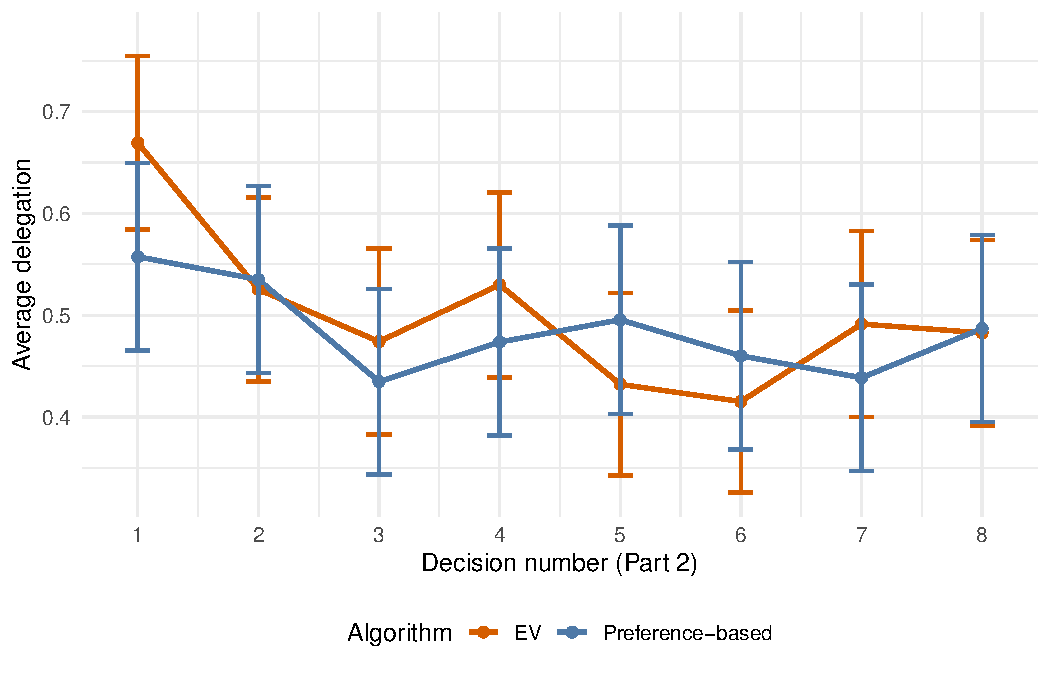
\includegraphics[width=0.8\textwidth]{Figure1_AverageDelegation.pdf}
\caption{Average Delegation Over Decisions}
\label{fig:over_time}
\end{figure}

\begin{figure}[htbp]
\centering
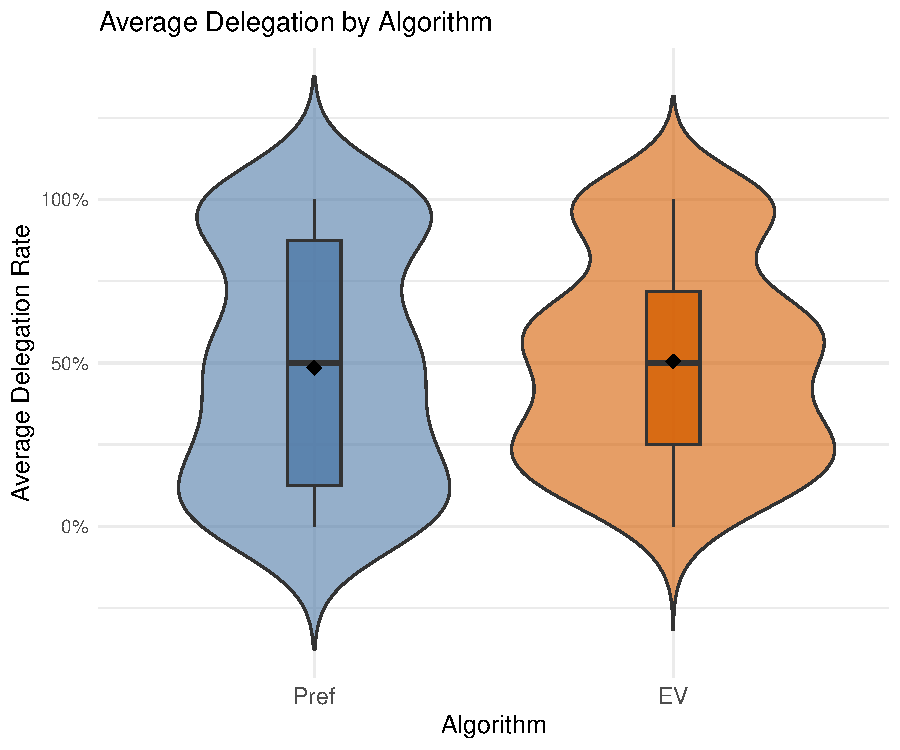
\includegraphics[width=0.8\textwidth]{Figure2_DistributionDelegation.pdf}
\caption{Distribution of Average Delegation}
\label{fig:distribution}
\end{figure}

\begin{figure}[htbp]
\centering
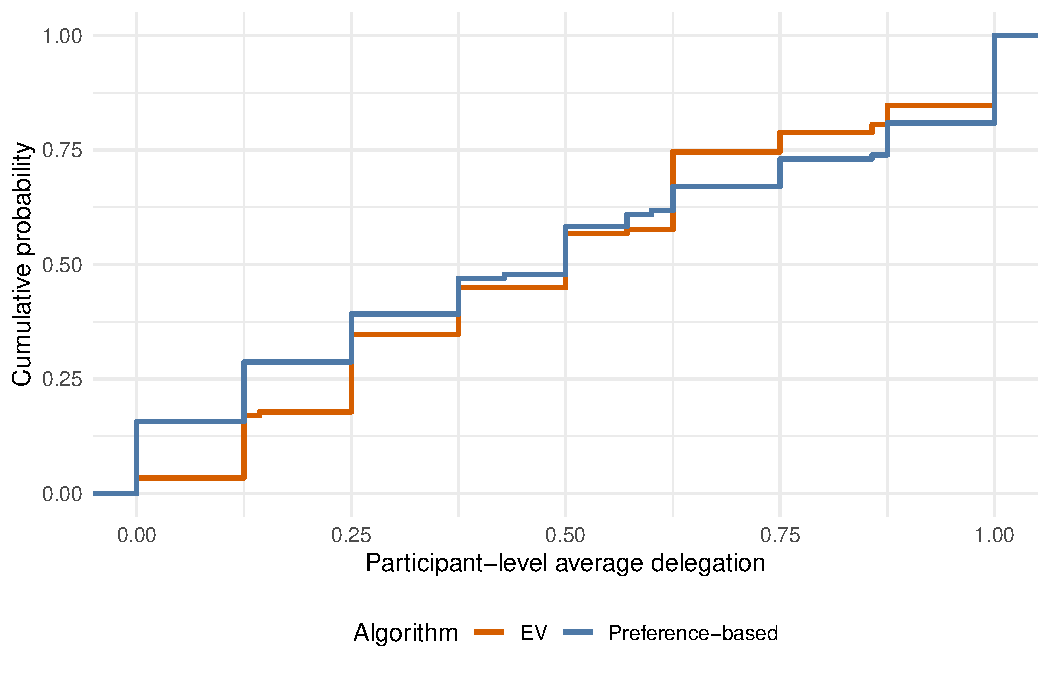
\includegraphics[width=0.8\textwidth]{Figure3_ECDF.pdf}
\caption{ECDF of Average Delegation}
\label{fig:ecdf}
\end{figure}

\begin{figure}[htbp]
\centering
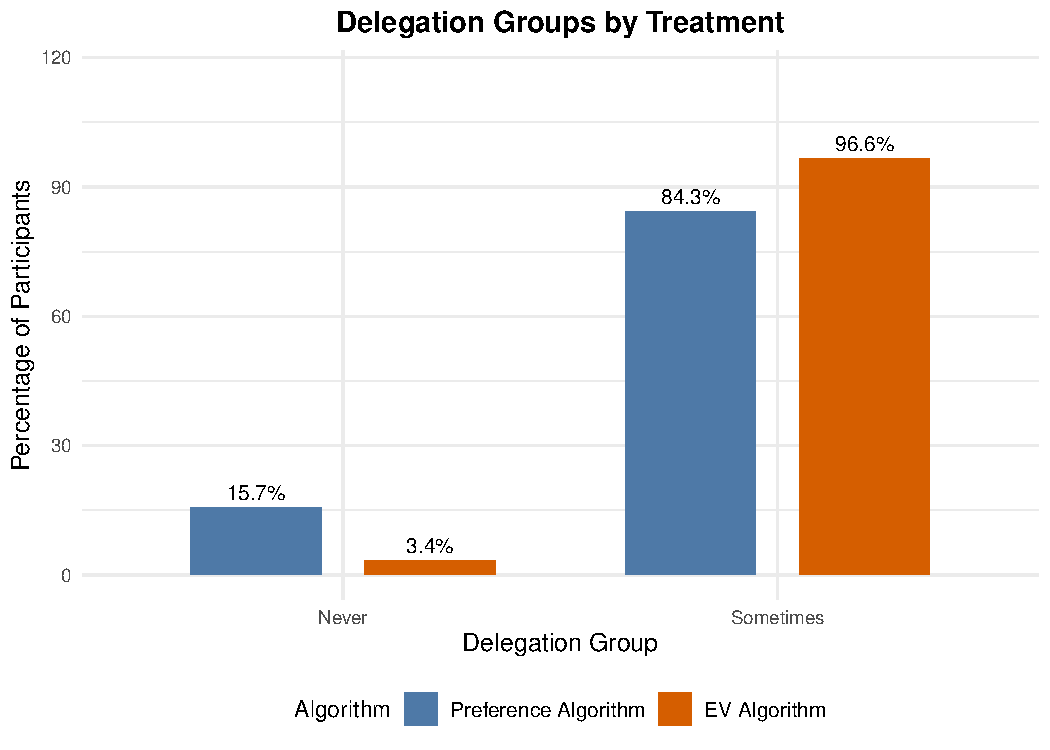
\includegraphics[width=0.8\textwidth]{Figure4_DelegationGroups.pdf}
\caption{Delegation Groups by Treatment}
\label{fig:groups}
\end{figure}

\begin{figure}[htbp]
\centering
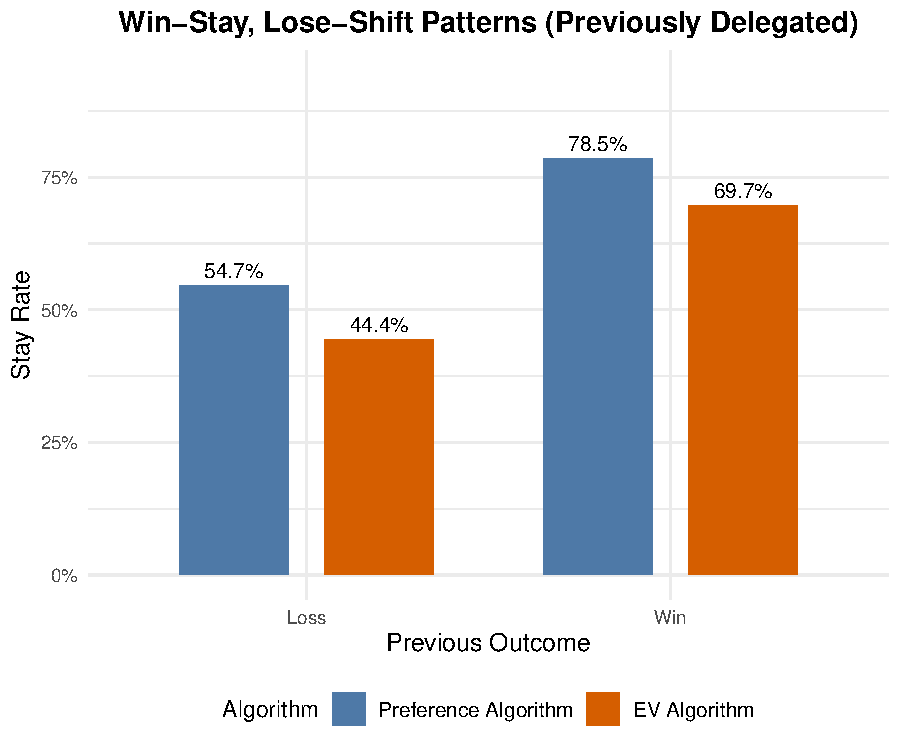
\includegraphics[width=0.8\textwidth]{Figure5_WinStayLoseShift.pdf}
\caption{Win-Stay, Lose-Shift Patterns}
\label{fig:win_stay}
\end{figure}

% Discussion
\section{Discussion}
\label{sec:discussion}
\section{Discussion}

\subsection{Main Findings}

This preregistered experiment provides novel evidence that personalization can deter rather than encourage delegation to algorithms. Participants delegated significantly more to an EV-maximizing algorithm than to a personalized algorithm that incorporated their individual preferences in the first decision (66.9\% vs. 55.8\%, p = 0.0413). However, this difference did not persist in subsequent decisions (p = 0.4413). This counterintuitive finding challenges common assumptions about the benefits of personalization in AI systems and has important implications for the design of algorithmic advisors.

\subsection{Theoretical Implications}

\subsubsection{Algorithm Appreciation vs. Aversion}

Our findings contribute to the ongoing debate about algorithm aversion and appreciation \citep{dietvorst2015, logg2019}. While \citet{logg2019} found that people prefer algorithmic judgment over human judgment in objective tasks, and \citet{dietvorst2015} showed that people avoid algorithms after observing errors, our results suggest that the type of algorithm matters. Participants initially preferred an objective EV algorithm over a personalized algorithm, even though the personalized algorithm should theoretically lead to higher expected utility for them.

This finding aligns with \citet{castelo2019}, who showed that algorithm aversion/appreciation depends on task type (objective vs. subjective). In our study, the EV algorithm may have been perceived as more objective and competent, while the personalized algorithm may have been perceived as more subjective and potentially less reliable.

\subsubsection{Role of Personalization in Trust}

Our results challenge the assumption that personalization always increases trust in AI systems. While \citet{longoni2019} found that personalization increases trust in medical AI, and \citet{jussupow2020} suggested that personalization can reduce aversion when AI accounts for unique situations, our study shows that personalization can actually deter delegation in certain contexts.

One possible explanation is that participants may have perceived the EV algorithm as more competent and reliable because it maximizes expected value, which is an objective criterion. In contrast, the personalized algorithm may have been perceived as less transparent or less trustworthy because it incorporated subjective preferences. This aligns with \citet{hoff2015}, who found that perceived competence is a key factor influencing trust in automation.

\subsubsection{MABA-HABA Framework}

Our findings can be interpreted through the MABA-HABA (Machines Are Better At vs. Humans Are Better At) framework proposed by \citet{glikson2020}. The EV algorithm aligns with the MABA principle, as it excels at objective calculations and expected value maximization. The personalized algorithm, however, blurs the boundary between what machines are better at and what humans are better at, potentially creating confusion about the appropriate division of labor.

\subsubsection{Trust and Reliance}

Our study distinguishes between trust as an attitude and reliance as behavior \citep{lee2004}. While we did not directly measure trust attitudes, our behavioral measures of reliance show that participants were less willing to rely on the personalized algorithm, at least initially. This aligns with \citet{kohn2021}, who emphasized the importance of measuring both trust attitudes and reliance behaviors.

\subsection{Practical Implications}

\subsubsection{AI System Design}

Our findings have important implications for the design of AI systems, particularly in financial advising. Designers should carefully consider when to personalize recommendations and when to use objective algorithms. In contexts where objective criteria are available and valued, such as expected value maximization in financial decisions, objective algorithms may be more trusted and more likely to be used.

\citet{holzmeister2023} found similar patterns in delegation to financial advisors, suggesting that our findings may generalize to real-world financial decision-making contexts. Designers of robo-advisors should consider whether personalization enhances or detracts from perceived competence and trustworthiness.

\subsubsection{User Education and Communication}

Our results suggest that users may not fully understand the benefits of personalized algorithms. From an economic perspective, the personalized algorithm should be preferred because it incorporates revealed preferences and leads to higher expected utility. However, participants initially chose the objective EV algorithm, suggesting a misunderstanding of the algorithm's benefits.

This highlights the importance of user education and transparent communication about algorithm capabilities and limitations. \citet{leightmann2023} found that explainability affects trust in AI, and \citet{ning2024} showed that transparency affects advice utilization. Designers should clearly communicate how personalized algorithms work and why they may be beneficial for users.

\subsubsection{Policy and Regulation}

Our findings also have implications for policy and regulation of AI-assisted decision-making. Regulators should consider that personalization may not always increase trust or adoption of AI systems. Guidelines for AI-assisted decision-making should emphasize transparency about algorithm type and expected outcomes, and should encourage designers to carefully consider the trade-offs between personalization and objectivity.

\subsection{Limitations}

\subsubsection{Experimental Design}

Our study has several limitations. First, it was conducted online with limited stakes, which may affect the generalizability of our findings. While participants received real monetary payments, the amounts were relatively small, and the decisions were hypothetical in the sense that participants did not have real money at risk.

Second, our study focused on a specific domain (lottery choices) and a specific type of decision (financial risk-taking). The extent to which our findings generalize to other domains (e.g., medical decisions, hiring decisions) is unclear and should be examined in future research.

Third, our sample consisted of UK residents recruited from the Prolific platform, which may not be representative of the broader population. Cultural factors may influence trust in AI and delegation behavior, and our findings may not generalize to other cultural contexts.

\subsubsection{Measurement}

We did not directly measure trust attitudes or perceived competence, relying instead on behavioral measures of reliance. While this aligns with the distinction between trust and reliance \citep{lee2004}, future research should include both attitudinal and behavioral measures to provide a more complete picture.

We also did not measure participants' understanding of the algorithms or their perceptions of algorithm competence. Future research should examine these factors to better understand the mechanisms underlying our findings.

\subsubsection{One-Shot Interaction}

Our study involved a one-shot interaction with the algorithms, with no long-term relationship or repeated interactions. In real-world settings, users may develop trust in algorithms over time through repeated interactions. Future research should examine how delegation behavior changes over longer time horizons and with repeated interactions.

\subsection{Future Research}

\subsubsection{Mechanisms}

Future research should investigate the mechanisms underlying our finding that personalization deters delegation. Why do participants initially prefer objective algorithms over personalized ones? Is it due to perceived competence, transparency, or some other factor? Experimental manipulations of these factors could help identify the causal mechanisms.

\subsubsection{Design Interventions}

Future research should test interventions to increase trust in personalized algorithms. For example, would providing explanations of how the personalized algorithm works increase delegation? Would highlighting the benefits of personalization (e.g., higher expected utility) increase adoption? \citet{shin2021} found that explainability and causability affect trust in human-AI collaboration, suggesting that such interventions may be effective.

\subsubsection{Extensions}

Future research should extend our findings to other domains and contexts. Would similar patterns emerge in medical decision-making, hiring decisions, or other domains where personalization is common? \citet{longoni2019} found that personalization increases trust in medical AI, suggesting that domain-specific factors may moderate the effects of personalization.

Future research should also examine cross-cultural differences in delegation to algorithms. Cultural factors may influence trust in AI and preferences for personalization, and our findings may not generalize to all cultural contexts.

\subsubsection{Longitudinal Studies}

Future research should conduct longitudinal studies of delegation over time. How does delegation behavior change as users gain more experience with algorithms? Do users learn to trust personalized algorithms over time? Longitudinal studies could provide insights into the dynamics of trust and reliance in human-AI collaboration.

\subsection{Conclusion}

This preregistered experiment provides novel evidence that personalization can deter rather than encourage delegation to algorithms. Participants initially delegated more to an objective EV algorithm than to a personalized algorithm, even though the personalized algorithm should theoretically lead to higher expected utility. This counterintuitive finding challenges common assumptions about the benefits of personalization in AI systems and has important implications for the design of algorithmic advisors.

Our results contribute to the literature on algorithm appreciation, trust in AI, and human-AI collaboration. They suggest that in certain contexts, particularly those involving objective calculations, people may prefer algorithms that are perceived as competent and objective rather than those that attempt to personalize recommendations. This has practical implications for the design of AI systems in finance and other domains where delegation decisions are important.

Future research should explore the mechanisms underlying this effect and test interventions to optimize the balance between personalization and trust. As AI continues to play an increasing role in decision-making, understanding when and why people delegate to algorithms will be crucial for designing systems that are both effective and trusted.

% Conclusion
\section{Conclusion}
\label{sec:conclusion}
\section{Conclusion}

This preregistered experiment examined how personalization affects delegation to algorithms in financial decision-making. We found that participants initially delegated more to an objective EV-maximizing algorithm than to a personalized algorithm that incorporated their individual preferences (66.9\% vs. 55.8\%, p = 0.0413). However, this difference did not persist in subsequent decisions (p = 0.4413). A large proportion of participants (75.1\%) never delegated to either algorithm.

Our findings challenge common assumptions about the benefits of personalization in AI systems. While personalization is often assumed to increase trust and adoption, our results show that it can actually deter delegation in certain contexts. Participants initially preferred an objective algorithm over a personalized one, even though the personalized algorithm should theoretically lead to higher expected utility for them.

This counterintuitive finding has important implications for the design of algorithmic advisors. Designers should carefully consider when to personalize recommendations and when to use objective algorithms. In contexts where objective criteria are available and valued, such as expected value maximization in financial decisions, objective algorithms may be more trusted and more likely to be used.

Our study also highlights the importance of user education and transparent communication about algorithm capabilities and limitations. Users may not fully understand the benefits of personalized algorithms, and designers should clearly communicate how these algorithms work and why they may be beneficial.

Future research should investigate the mechanisms underlying our finding that personalization deters delegation, test interventions to increase trust in personalized algorithms, and examine whether our findings generalize to other domains and cultural contexts. As AI continues to play an increasing role in decision-making, understanding when and why people delegate to algorithms will be crucial for designing systems that are both effective and trusted.

In conclusion, our study provides novel evidence that personalization can deter rather than encourage delegation to algorithms, challenging common assumptions about the benefits of personalization in AI systems. This finding contributes to the literature on algorithm appreciation, trust in AI, and human-AI collaboration, and has important practical implications for the design of algorithmic advisors in finance and other domains.

% References
\bibliographystyle{apalike}
\bibliography{references}

% Appendices
\appendix

\section{Additional Regression Tables}
[Additional regression results]

\section{Experimental Materials}
[Instructions, example lottery choices, questionnaire items]

\section{Additional Analyses}
[Detailed never-delegator analysis, win-stay/lose-shift by individual, correlation matrices]

\section{Preregistration Document}
[Link to AsPredicted registration, deviations from preregistration]

\end{document}